%%%%%%%%%%%%%%%%%%%%%%%%%%%%%%%%%%%%%%%%%
% Journal Article
% LaTeX Template
% Version 1.4 (15/5/16)
%
% This template has been downloaded from:
% http://www.LaTeXTemplates.com
%
% Original author:
% Frits Wenneker (http://www.howtotex.com) with extensive modifications by
% Vel (vel@LaTeXTemplates.com)
%
% License:
% CC BY-NC-SA 3.0 (http://creativecommons.org/licenses/by-nc-sa/3.0/)
%
%%%%%%%%%%%%%%%%%%%%%%%%%%%%%%%%%%%%%%%%%

%----------------------------------------------------------------------------------------
%	PACKAGES AND OTHER DOCUMENT CONFIGURATIONS
%----------------------------------------------------------------------------------------

\documentclass[twocolumn]{article}

\usepackage{blindtext} % Package to generate dummy text throughout this template 

\usepackage[sc]{mathpazo} % Use the Palatino font
\usepackage[T1]{fontenc} % Use 8-bit encoding that has 256 glyphs
\linespread{1.0} % Line spacing - Palatino needs more space between lines
\usepackage{microtype} % Slightly tweak font spacing for aesthetics


\usepackage[english]{babel} % Language hyphenation and typographical rules

\usepackage[hmarginratio=1:1,top=32mm,columnsep=20pt]{geometry} % Document margins
\usepackage[hang, small,labelfont=bf,up,textfont=it,up]{caption} % Custom captions under/above floats in tables or figures
\usepackage{booktabs} % Horizontal rules in tables

\usepackage{lettrine} % The lettrine is the first enlarged letter at the beginning of the text
\usepackage[titletoc,toc,title]{appendix}

\usepackage{enumitem} % Customized lists
\setlist[itemize]{noitemsep} % Make itemize lists more compact

\usepackage{abstract} % Allows abstract customization
\renewcommand{\abstractnamefont}{\normalfont\bfseries} % Set the "Abstract" text to bold
\renewcommand{\abstracttextfont}{\normalfont\small\itshape} % Set the abstract itself to small italic text

\usepackage{titlesec} % Allows customization of titles
\renewcommand\thesection{\Roman{section}} % Roman numerals for the sections
\renewcommand\thesubsection{\roman{subsection}} % roman numerals for subsections
\titleformat{\section}[block]{\large\scshape\centering}{\thesection.}{1em}{} % Change the look of the section titles
\titleformat{\subsection}[block]{\large}{\thesubsection.}{1em}{} % Change the look of the section titles

\usepackage{fancyhdr} % Headers and footers
\pagestyle{fancy} % All pages have headers and footers
\fancyhead{} % Blank out the default header
\fancyfoot{} % Blank out the default footer
\fancyhead[C]{Practical MA-ABE for Secure Cloud Strogae Systems $\bullet$ August 2018 $\bullet$ Vol. I, No. 2} % Custom header text
\fancyfoot[EL]{\thepage} % Custom footer text

\usepackage{titling} % Customizing the title section

\usepackage{hyperref} % For hyperlinks in the PDF
\usepackage{multicol}
\usepackage{graphicx}
\usepackage{caption}
\usepackage[textsize=footnotesize]{todonotes} % for todo notes

%----------------------------------------------------------------------------------------
%	TITLE SECTION
%----------------------------------------------------------------------------------------

\setlength{\droptitle}{-4\baselineskip} % Move the title up

\pretitle{\begin{center}\Huge\bfseries} % Article title formatting
\posttitle{\end{center}} % Article title closing formatting
\title{Practical Multi-Authority Attribute-Based Encryption Scheme for Secure Cloud Storage Systems } % Article title
\author{%
\textsc{Marvin Petzolt}\\[1ex] % Your name
\normalsize TU Berlin \\ % Your institution
\normalsize \href{mailto:marvin.petzolt@protonmail.com}{marvin.petzolt@protonmail.com} % Your email address
%\and % Uncomment if 2 authors are required, duplicate these 4 lines if more
%\textsc{Jane Smith}\thanks{Corresponding author} \\[1ex] % Second author's name
%\normalsize University of Utah \\ % Second author's institution
%\normalsize \href{mailto:jane@smith.com}{jane@smith.com} % Second author's email address
}
\date{\today} % Leave empty to omit a date
\renewcommand{\maketitlehookd}{%
\begin{abstract}
If a group of users want to share a ciphertext, they need to agree on a shared key. On each leave or join of a user this shared key needs to be updated for each user to ensure forward secrecy. Classical encryption reaches the point where this approach is no longer feasible for a large number of users. In this work the field of attribute based encryption (ABE) will be analyzed to solve this issue for a secure cloud storage environment (Bdrive). Different ABE schemes will be compared and analyzed for their applicability in Bdrive. In the end the implementation of the resulting scheme will be evaluated for performance, scalability and security.
\end{abstract}
}

%----------------------------------------------------------------------------------------

\begin{document}

% Print the title
\twocolumn[
    \maketitle
]


%----------------------------------------------------------------------------------------
%	ARTICLE CONTENTS
%----------------------------------------------------------------------------------------

\section{Introduction}
\label{sec:introduction}
\lettrine[nindent=0em,lines=3]{I}n public-key cryptography each user is identified by his unique public and private key pair. Peer-to-peer communication works well with this scheme, but as soon as an encrypted content needs to be accessed by multiple participants, the data owner has to encrypt the content for each user explicitly. This results in many encrypted versions of the same  file, each secured by a different public key. Such scheme does not scale in the secure cloud storage domain. Here often data holders want to share the same content with many other users at the same time.

We reach the point where the classical public-key end-to-end encryption scheme does not scale anymore. We would like to employ an encryption scheme which has a constant number of access keys regardless of the number of participants.

\section{Related Work}
In the following we will describe the encryption scheme currently enrolled in Bdrive and give an rough overview of the existing solutions in the attribute-based encryption domain.

\subsection{Background}
Bdrive is a secure cloud storage which splits up files in smaller chunks that are saved separately on different cloud storage provider (CSP). To ensure end-to-end encryption a Bdrive client encrypts locally each of its chunks with a one-time symmetric key that is than encrypted under its own public key. This encrypted key is called a file key and it is uploaded to the Bdrive server where it is stored securely (see figure \ref{fig:filekey}).

Since each device of the same user has a different private-public key pair, the device is in charge of making the file keys available for a new device. This is done by downloading each file key for the respectiv file, receiving the public key of the new device, decrypting the file key with its own private key, encrypting it again with the public key of the new device and finally, uploading the new file key to the Bdrive server. This process will be called re-keying. (see figure \ref{fig:rekey})

The number of file keys, that need to be maintained in Bdrive, grows linearly with the number of devices. In addition Bdrive allows to share files between different users. For each device of each user involved in the sharing a new file key has to be created and maintained. 

%The formula \ref{eq:rekey} describes the number of file keys Bdrive that need to be stored for each shared files between $U$ users, where each user $u_{i \in U}$ has $u_d$ devices.

%\begin{equation}
%n = \sum_{i}{d_i}
%\label{eq:rekey} 
%\end{equation}

%Lets construct an example where the manager of a company wants to create a shared folder with all company employees. It is a medium sized company with $50$ employees. Lets assume that at least haft of them have two Bdrive clients running. The manager wants to upload the $250$ photos of the last company trip.
%We end up by computing $3/2 * 50 * 250 = 18750$ file keys and for every new file uploaded $75$ new file keys need to be uploaded. 




\subsection{Attribute-Based Encryption}
Attribute Based Encryption (ABE), first introduced by Sahai and Waters \cite{sahai2005fuzzy}, is a cryptographic encryption scheme which encrypts under attributes that describe a user. This enables the data owner to craft a ciphertext over chosen attributes that can only be decrypted by any entity that holds a super set of matching attributes. Further, it is possible to embed an complex access structure (e.g. access trees) inside the cipher text, where each node contains \textit{AND} or \textit{OR} threshold gates. This approach is known as Ciphertext-Policy Attribute-Based Encryption (CP-ABE) \cite{bethencourt2007ciphertext}. 
It is also possible to do it the other way around: Associate the user's key with an access policy. Formally known as Key-Policy Attribute Based Encryption (KP-ABE).\cite{goyal2006attribute}. 
%Now the encryptor needs only to encrypt a given plain text with the public key of specific attributes so that only users who hold the right keys are able to decrypt the cipher text.

Both approaches are limited to one attribute authority (AA). So only one trusted entity is in charge of issuing attributes and their matching key pairs. However, in the real world we would like to distribute the issuing of attributes over different domains. A new scheme is needed where different attribute authorities cooperate and communicate across different domain.  

% The basic idea is, as proposed in \cite{chase2007multi}, to construct for each users a polynomial of degree $d-1$, where $d$ donates the number of attributes in our system. 

Multi-Authority Attribute Based Encryption (MA-ABE), first proposed by Chase 2007 \cite{chase2007multi}, allows multiple attribute authorities to maintain different attribute domains. To ensure collusion resistance between users, a trusted  central authority (CA) was introduced to assign each user an unique identifier (UID) and making the decryption process depending on this UID. The disadvantage of this scheme was that the CA had global decryption power and so has to remain trusted. 
%To prevent collusion between user in a multi authority setting, the challenge for each user needs to be individual. But it still needs to be ensured that the encryption of a message is independent of any user specific identifier, since the encryption progress should sourly depend on the attribute set known to the system.
%To mitigate this problem a global identifier (GID or UID) per users was introduced that is shown to each attribute authority (AA) to receive the corresponding private key for the users attributes. 
%The central authority (CA) now has to make sure that the user dependent challenge results in a global decryption key to decrypt the message.
%In fact the CA has to be trusted since it computes the users private keys in such a way that on decryption it reveals the global decryption key. 
Chase addressed this issue in \cite{chase2009improving} by distributing the global secret  master key generation over the AAs. However, since the global master secret is computed on system initialization, no more AAs can be added afterwards without rebooting the system. Also the scheme did not support attribute revocation which rendered it practical not applicable.
% Each authority uses this seed in combination with a pseudo random function to deterministically create the users private key. Since the CA possesses the same seed, same pseudo random function and issues the users GID, it can also compute the same private key as issued by the corresponding AA. So it can ensure that on decryption the keys add up to reveal the global decryption key. This scheme has a major issue: The CA has global decryption power. 

% Chase notices this problem as well and tried to mitigate it by decentrializing the seed generation \cite{chase2009improving}.  First user attributes could not easly be revoked\footnote{Chase proposed to assign each user a range of GIDs, so that a user can migrate to the next GID on revocation. Since the GID range is finite, this solution does not scale.}. Second AA's cant be added on runtime without reissuing each user his keys. And last, the attribute universe is finite (no large-universe). Further we noticed that if a failure of one AA renders the system unresponsible, since a cyphertext includes attributes from each authority. 

Data Access Control for Multi-Authority Cloud Storage systems (DAC-MACS) \cite{yang2013dac} is a scheme that tackles both of this issues. Each authority receives its own ciphertext that dependents solely on the attributes issued in this domain. While Chase managed to maintain "one-plaintext-one-ciphertext", DAC-MACS needs to create $k$ ciphertexts: One per attribute authority.\footnote{If the ciphertext does not require any attributes of an specific authority it does not have to create a ciphertext for this domain.} DAC-MACS does not require any coordination between authorities which enables to add new authorities at runtime without recreating the user keys. This scheme also includes features for efficient revocation while it claimed to maintain forward and backward secrecy. 

DAC-MACS was not collusion resistance on attribute revocation under the active attack model. The scheme NEDAC-MACS (New Extended DAC-MACS) showed and solved the vulnerability \cite{wu2017security}. Recent studies introduced a more efficient, scalable and secure approaches such as MAACS \cite{li2016secure} and TFDAC-MACS (Two-Factory DAC-MACS)\cite{li2017two}. The DAC-MACS family is further known for the proxy decryption technique, first introduced by \cite{li2013matrix}, where a honest-but-curious server helps the user on decryption.

Priscilla and Nagarajan 2018 \cite{nagarajan2018overview} conducted an analysis of the DAC-MACS family. In addition to that work, this thesis will focus on alternative approaches to improve scalability of secure cloud storage systems and analyse the field of ABE and MA-ABE more deeply.   



%------------------------------------------------

\section{Requirements}
\label{sec:requirements}
The general requirements of this thesis will be summarized by two major points: 

\begin{itemize}
	\item \textbf{Performance:} Participating in the system should also be possible with low-performance devices (such as smartphones). The overhead for the server on proxy decryption, attribute issuing and revocation should be reasonably low.  
	\item \textbf{Scalability:} The system should scale better than the current encryption scheme with respect to the number of file keys. 
\end{itemize}

In addition, the core security requirements in the context of an MA-ABE scheme are the following:
\begin{itemize}
\item \textbf{Collusion resistance:} For two users it should not be possible to combine their attributes to archive a higher level of decryption power.
\item \textbf{Inter-Company Sharing:} Each company is only responsible for its own domain. This includes attribute and user administration, which translates to secret key generation and revocation. %Since Bdrive would need to consider a multi-authority ABE scheme, it should not be possible for a company to decrypt or issue files of other companies if no explicit exception is given for certain files by a trusted company relationship. A companies attribute authority (AA) should be responsible for its domain. In the case of an inter company relationship, attributes needs to be issued across different companies. 
\item \textbf{Central Authority:} The CA shall not have global decryption power. At most an AA can decrypt user files of its own domain.  
\item \textbf{Secret Master key (if any):} Key recovery requires a secret and securely stored master key. It should solely function in the company domain and not globally. 
\item \textbf{Large Attribute and Key Universe:} The number of attributes and users shall not be restricted.
\item \textbf{Adding new Attribute Authorities:} It should be possible to add new attribute authorities at runtime. Without either shutting down the system or recreating each key.
\item \textbf{Untrusted Attribute Authority:} A corrupt Attribute Authority can only harm its own domain, but can not harm the outside system in any way. It can not gain any additional information.
\item \textbf{Key and Attribute revocation:} Revocation is needed to handle user management in terms of attribute promotion, attribute demotion and key revocation. Forward secrecy should be provided. 
\end{itemize}

\noindent Other (optional) requirements are: 
\begin{itemize}
	\item \textbf{Traitor tracing:} A user in ABE is described by his attribute set and is anonymous in this set. Misbehaving users, that sell their attribute keys to create a decryption black box, should be identifyable. \cite{liu2016practical}
	\item \textbf{Fine-granted access control:} The user shall not be bounded on defining fine-granted access policies which requires either an access tree \cite{bethencourt2007ciphertext} or an linear secret sharing scheme (LSSS) \cite{yang2013dac} \cite{li2016secure} \cite{wu2017security} \cite{li2013matrix} \cite{liu2016practical}.
	%Some schemes restrict the user to threshhold access policies, where an user needs at least $n$ of $m$ attributes to encrypt the cipher text. \cite{chase2007multi} \cite{chase2009improving} Other approaches are restriced to $AND$ gates which would translate to $m$ of $m$ threshhold gates. \cite{li2017two}
\end{itemize}

\section{Targets}
The target of this work is to find a more scalable solution to the current enrolled re-keying scheme in Bdrive. The new scheme needs to satisfy the requirements of section \ref{sec:requirements} with respect to multi-company management (each company administrates only its own domain) and inter-company file sharing (it is possible to share files across companies), as well as it should be practical applicable in the real world.

%------------------------------------------------
 
\section{Concept}
In detail this work splits into two parts. In the theoretical part (minimal requirement) related work is analyzed with respect to the requirements. It will be evaluated, whether ABE is the best solution currently available to the scalability problem in the secure cloud storage domain. More deeply will the topic of ABE be analyzed. Here the goal is to find or construct the best matching security scheme. This approaches will be evaluated with respect of scalability, performance and security. The security requirements of section \ref{sec:requirements} need to be satisfied by the selected approach. If no matching related work is found, that fully satisfy the requirements, different approaches will be combined to create a new security scheme.\\

\noindent \textbf{Theoretical part:}
\begin{enumerate}
	\item\textbf{Evaluation of alternative security schemes.} \textit{(2 weeks)} \\
		  %First it needs to be clarified, if ABE is the right tool to countermeasure the scalability problem of Bdrive. Hence, different related security schemes shall be evaluated and compare to each other. 
		  %The scalability issue for large group communication is not new. 
		  %Several approaches exist to make the re-keying process for group members more efficient. 
		  %This schemes are called secure group communications and create a more efficient re-keying scheme.
		  Argumentatively ABE will be compared to different promising schemes (e.g. secure group communications \cite{wong2000secure}) (at most 2) and based on scalability, performance and security a decision should be made. 
		  Other compare metrics could be the number of resulting file keys and the maintaining overhead of the re-keying process. 

	%\makebox[\columnwidth]{$\vcenter{\hbox{\rule{0.38\columnwidth}{0.7pt}}}$  Option 1. $\vcenter{\hbox{\rule{0.38\columnwidth}{0.7pt}}}$}
	\item\textbf{Evaluation of ABE schemes.} \textit{(5 weeks)} \\
		  To compare different ABE approaches, a homogeneous platform needs to be created. With this platform the different approaches can be implemented and compared regarding scalability (number of users, number of attributes, number of resulting ciphertexts, number of keys that need to be stored). Here tools like CloudSim\footnote{\url{http://www.cloudbus.org/cloudsim/}} or docker\footnote{\url{https://www.docker.com/}} may help on simulating the different scenarios. To reduce the number of possible candidates, the ABE paper will be clustered into topics and a representing candidate will be chosen. If an reference implementation is given this implementation will be translated into the homogeneous environment. Otherwise an implementation has to be written. 
		  The target of this section will be to construct a comparable environment of different ABE approaches and to create an overview table containing different features and the matching requirements.

	\item\textbf{Evaluation of MA-ABE schmes.} \textit{(5 weeks)} \\  
		  If the result of the previous section would be that MA-ABE schemes fit best, the next step would be to construct an deeply analysis of the different MA-ABE schemes. This will happen in the same way as in the previous section. Here can also the number of attribute authorities be varied to evaluate the scalability of the respective scheme. 
		  The conclusion describes either a well argued approach extracted from a paper or a self designed scheme if the related work is missing some requirements. In the case this section yields an own constructed scheme, this scheme needs to be proven secure.  
\end{enumerate}

If an early stage of analysis leads to constructing an own approach the theoretical part will be reordered as following: Evaluation of alternative security schemes (2 weeks), evaluation of ABE and MA-ABE schemes (4 weeks\footnote{Evaluation time will be shortened to leave more space to construct a new scheme}) and finally constructing, proofing, comparing and evaluating the new security scheme against related schemes (6 weeks). 
The last part will be done in similar ways as described above: A homogeneous platform will be created where a prototype of this approach can be compared against existing, related schemes. Especially performance can be evaluated by varying the number of AAs, the number of attributes and measuring the time for en- and decryption.\\
	%\makebox[\columnwidth]{$\vcenter{\hbox{\rule{0.38\columnwidth}{0.7pt}}}$  Option 2. $\vcenter{\hbox{\rule{0.38\columnwidth}{0.7pt}}}$}

\noindent \textbf{Practical part:}
\begin{enumerate}
	\item\textbf{Implementation of selected scheme} \textit{(4 weeks)}\\
		  The extracted scheme of the theoretical part will be implemented in detail. If an reference implementation is given this implementation will be used. If no implementation is given the goal is to create a prototype cryptographic library. To construct a comparable scheme like Bdrive a prototype file sharing system needs to be implemented that acts in an similar ways as Bdrive does (regarding (inter-company) sharing and file key creation). 

		  If an practical and usable implementation for this scheme already exists, ABE will be evaluated for practical usage. Recent paper analyzed practical ABE in the medical domain. \cite{thatmann2016please} \cite{li2013scalable} \cite{akinyele2011securing} Similar research shall be done for the secure cloud storage domain. It should be evaluated where to extract the attributes to solve the bootstrapping problem and how end users benefit from the new security scheme. Further, this scheme will be tested for usability, performance, real-world scalability. The central question would be if real-world use-cases exist where ABE can clearly out-perform classical public-key encryption.

	\item\textbf{Evaluation of implementation} \textit{(2 weeks)}\\
		  Finally we want to compare the new implementation to the existing one in Bdrive. Here performance and scalability evaluations about the number of file keys, the computing time for en- and decryption as well as attribute revocation will be conducted and compared to the classical re-keying scheme.
		  % As introduced in section \ref{sec:introduction} the main target is to make Bdrive more scalable. This will be done by evaluating a new crytographic scheme that reduces the number of file keys that need to be maintained per file. 
		  %With MA-ABE we expect to reduce the number of file keys per file to at least $n = k$. Where $k$ is the number of attribute authorities and assuming that we don't have revoced attributes yet. 
		  %Since computing pairing requires a bigger overhead than computing the power of a prime as in RSA, we need to compare the time it takes to encryt the file key. To show that MB-ABE is indeed faster we would compare this time for an increasing number of devices. While we expect to DAC-MACS's comuting time to remain constant on encrypting for a increasing number of devices, we expect a linear increasing function for RSA. 
		  
	\item\textbf{Summarzing results} \textit{(6 weeks)}\footnote{The master thesis is restricted to 26 weeks in total. The remaining two weeks are mend as a buffer for unexpected difficulties or delays.}\\
		  The remaining time will be used to write the thesis and collect the results.   
\end{enumerate}

% --------------------------- DAC-MACS -------------------------

%For the design of the Bdrive MA-ABE scheme the paper \cite{yang2013dac} will be used. Here the encryptor encrypts for each attribute authority the ciphertext with the required attributes, so that he endups with $k$ cyphertext, one for each authority. So DAC-MACS breaks the "one-plaintext-one-ciphertext" contains, but makes the AAs independent from each other. This is the mayjor difference between DAC-MACS (\cite{yang2013dac}) and chases multi-authority proposals (\cite{chase2007multi}, \cite{chase2009improving}). DAC-MACS comes also with a handfull of security features that are requirements of Bdrive as proposed in section \ref{sec:requirements}. The scheme consist of three entities:

%\begin{itemize}
%\item \textbf{Certificate Authority (CA)}: Issues users global identifier (UID) to make the user distinglishable and prevent collusion. It signs the users arttibutes such as the Public key, UID and other user specific security paramter. 
%\item \textbf{Server}: The server helps the user by decryption the cyphertext and re-encryption his cyphertexts on attribute revocation. The server does not have global knowledge over the ciphertext, since it decrypts first to a decryption token, that can only be decyrpted by the users privat key. 
%\item \textbf{Attribute authority (AA)}: Each AA is responsible for their own domain attributes. They generate independenlty thier own secret and public key components and issue the user his attributes. Each attribute key is verioned, so that for revocation the AA simply needs to increase the version number and reissue the user his keys. The user hisself need than to update the cyphertexts. 
%\end{itemize}

%DAC-MACS fits the security requirements of Bdrive quite well. In the following each requirement will be analysed and dicussed how DAC-MACS solves this problem. 

%\begin{itemize}
%\item \textbf{Collusion resistance:} This is the key requirement of each ABE scheme. In a Multi-Authority setting we need to additional ensure collusion resistance between users of different authorities. In DAC-MACS this is done in the classical way as also in other Multi-Authroity schemes: By using global unique user identifier. They are presented to each authority in exchange of the users secret attribute keys. This secret keys contain the user public key component so that on decryption the attribute specific ciphertext first resolves into the another ciphertext that can only be decyrpted with the users privat key. As argumented collusion resistance is ensured in that way that if users would combine their secret keys of an attribute key are not able to archive a higher level of decyrption power since the attribute specific ciphertext will resolved in an undecryptable cipher text.  
%\item \textbf{Inter-Company Sharing:} This requirements is given by nature of an multi-authority scheme. A user needs to obtain attributes from both, the own and the foreign authoritiy to encrypt ciphertext in thier domain.
%\item \textbf{Central Authority:} The certificate authority and the server are both serving as cental authorities. While the Server is only semi-tursted (honst-but-currious), the certificate authrotity need to be trusted since the global user id needs to be unique over multibe users. If this contains is not preserved collusion would be possible. The CA does also not have global decryption power since the user specific attribute keys dependt on the users public key, that is chosen by the user secretly. 
%\item \textbf{Secret Master key (if any):} Since each ciphertexts are encrypted under the public key of the attribute authority and do not depent on any specific user security paramters, the attribute authority can decrypt the ciphertext. However, it can not decrypt the cyphertext of other attribute authorities.  
%\item \textbf{Large Key Universe:} De- and encryption scales linearly with the number of attributes and authorities. Revoking attributes only affects the cipher text and keys that are associated with the revoked attributes. 
%\item \textbf{Adding new Attribute Authorities:} Since each attribute authoritiy issues it own independent keys, we can add new attribute authorities without re-encyprtion all cipher texts. 
%\item \textbf{Key and Attribute revocation:} Attribute keys are versioned to ensure forward-secrecy. Revocation also happens in a direct manner. Backward-security is ensured so that new keys can not decyrpt old cipher texts.  
%\end{itemize}

%The main scope is to reduce the number of rekeys that are used on scaling number of user and devices that access this file key. As mentioned before chase proposed a scheme that only needs to maintain one ciphertext per plaintext. But to act dynamically regarding Attribute Authorities additions, reduce the number of affected ciphertext re-encryptions, and provide an encryption process that does not need to involve all AAs known to the system, we need to split up the ciphertext per AA domain. Furhter, in chase scheme, we would also encounter the problem of DoS attacks where an AA can simply deny requrest and render the whole system unusable.  

%\todo[inline]{Explain how to evaluate and compare the ABE paper}



% --------------------------- MA-ABE chase -------------------------
%\begin{figure*}[!h]
%\begin{itemize}
	%\item \textbf{System}:\\
	%\textbf{Init}: Fix prime order groups $G$, $G$, bilinear map $e: G \rightarrow G$, and generator $g \in G$. Choose seeds $s_1, \dots, s_K$ for all %authorities. Also choose $y_0 , \{t_{k,i}\}_{k=1...K,i=1\dots n} \leftarrow Z_q$. \\
	%\textbf{System Public Key}: $Y_0 = e(g, g)^{y_0}$
	%\item \textbf{Attribute Authority} $k$: \\
	%\textbf{Auhtority Secret Key}: $s_k, t_{k, 1} \dots t_{k,n} $ \\
	%\textbf{Authority Public Key}: $ T_{k, 1} \dots T_{k, n}$ where $T_{k, i} = g^{t_{k,i}} $\\
	%\textbf{Secret Key for User } $u$: Let $y_{k,u} = F_{s_k}(GID)$. Choose random $d - 1$ degree polynomial $p$ with $p(0) = y_{k,u}$. Secret Key: $\{D_{k%,i} = g^{p(i)/t_{k,i}} \}i \in A_u $.
	%\item \textbf{Central Authority}:\\
	%\textbf{Central Authority Secret Key}: $s_k$ for all authorities $k, y_0$.  \\
	%\textbf{Secret Key for User} $u$: Let $y_{k,u} = F_{s_k}(GID)$ for all $k$. Secret Key: $D_{CA} = g^{y_0 - \sum^K_{k=0} y_{k,u}}$
	%\item \textbf{Encryption for attributes set } $A_C$: \\
	%Choose random $s \leftarrow Z_q$. $E = Y_0^s m$, $E_{CA} = g^s$, $\{E_{k,i} = T^s_{k,i}\}_{i \in A^k_C, \forall k}$
	%\item \textbf{Decryption}:\\
	%For each authority $k$, for $d$ attributes $i \in A^k_C \cap A_u$, compute $e(E_{k,i}, D_{k,i}) = e(g,g)^{p(i)s} = e(g,g)^{y_{k,u}s}$.  Interpolate to find $Y^s_{k,u} = e(g, g)^{p(0)s} = e(g,g)^{y_{k,u}s}$ for each authority $k$. Compute $Y^s_{CA} = e(E_{CA} , D_{CA})$. Combine these values to obtain %$Y^s_{CA} * \prod^K_{k=1} Y^s_{k,u} = Y^s_0$. Then $m = E/Y_0^s$
%\end{itemize}
%\caption{Multi-Authority scheme as proposed by Chase 2007 in \cite{chase2007multi}. $A_u$ donates the attributes of user $u$. $A_C$ donates the attributes of the cipher text.}
%\label{fig:chase-multi-auth}
%\end{figure*}

%\begin{figure*}[!h]
%\begin{itemize}
	%\item \textbf{System}:\\
	%\textbf{Init}: Fix prime order groups $G$, $G$, bilinear map $e: G \rightarrow G$, and generator $g \in G$.

	%\item \textbf{Attribute Authority} $k$: \\
	%\textbf{Auhtority Secret Key}: $y_k \leftarrow Z_q$ (only used once), $s_{kj} = s_{jk}$ as exchanged with each authority $(k,j) \in (\{1 \dots N\} \%backslash \{k\}), t_{k, i} \leftarrow Z_q \forall i \in A_k$ \\
	%\textbf{Authority Public Key}: $Y_k = e(g,g)^{y_k}$, $ T_{k, 1} \dots T_{k, n}$ where $T_{k, i} = g^{t_{k,i}} $\\
	%\textbf{System Public Key}: Each authority computes $Y_0 = \prod Y_k = e(g, g)^{\sum y_k}$\\
	%\textbf{Secret Key for User } $u$: For $j \in \{1 \dots N\}\backslash \{k\}$: 
	%$Q_{kj} = g^{R_{kj}} * F_{s_{kj}}(GID)^{\delta_{kj}}$, $R_{kj} \leftarrow Z_q$ and set $\delta_{kj}$ to either $-1$ if $j<k$ otherwise $1$.

	%Choose random $d - 1$ degree polynomial $p$ with $p_k(0) = y_k - \sum_{j \in \{1 \dots N\} \backslash \{k\}} R_{kj}$. 

	%Secret Key: $\{D_{k,i} = g^{p(i)/t_{k,i}} \}i \in A_u $.

	%User computes: $Q_u = \prod_{(j,k) \in \{1 \dots N\} \times (\{1 \dots N\} \backslash \{k\})} Q_{kj} = g^{\sum_{(j,k) \in \{1 \dots N\} \times (\{1 \%dots N\} \backslash \{k\})} R_{kj}} = g^{R_u}$

	%\item \textbf{Central Authority}:\\
	%Issues unique $GID$ for user $u$.
	%\item \textbf{Encryption for attributes set } $A_C$: \\
	%Choose random $s \leftarrow Z_q$. $E = Y_0^s m$, $E_{1} = g^s$, $\{E_{k,i} = T^s_{k,i}\}_{i \in A^k_C, \forall k}$
	%\item \textbf{Decryption}:\\
	%For each authority $k$, for $d$ attributes $i \in A^k_C \cap A_u$, compute $e(E_{k,i}, D_{k,i}) = e(g,g)^{p(i)_{k}s}$.  Interpolate to find $P_k = e(g%, g)^{p(0)_{k}s} = e(g,g)^{s(y_k - \sum_{j \neq k} R_{kj})}$. Multiply $P_k$ together to get $V = e(g,g)^{s(\sum\{y_k\} -R_u)} = Y_0^s / e(g^{R_u}, g^{s})$. Compute $e(Q_u, E_1) * V = e(g^{R_u}, g^s) * V = Y_0^s$. Recover $m$ by $E/ Y_0^s$.
%\end{itemize}
%\caption{Multi-Authority scheme as proposed by Chase 2009 in \cite{chase2009improving}. $A_u$ donates the attributes of user $u$. $A_C$ donates the attributes of the cipher text.}
%\label{fig:chase-multi-auth-without-trusted-CA}
%\end{figure*}


%The basic idea is, as proposed in \cite{chase2007multi}, to construct for each users a polynomial of degree $d-1$, where $d$ donates the number of attributes in our system. 

%To prevent collusion between user in a multi authority setting, the challenge for each user needs to be individual. But we still need to ensure that the encryption of message is independent of any user specific identifier, since the encryption progress should sourly depend on the attribute set known to the system.
%To mitigate this problem a global identifier (GID) per users was introduced that is shown to each attribute authority (AA) to receive the corresponding private key for the users attributes. 
%The central authority (CA) now has to make sure that the user dependent challenge results in a global decryption key to decrypt the message.
%In fact the CA has to be trusted since it computes the users private keys in such a way that on decryption it reveals the global decryption key. 

%In \cite{chase2007multi} this is done by the CA generating random seeds that are distributed to the Attribute Authorities. Each authority uses this seed in combination with a pseudo random function to deterministically create the users private key. Since the CA possesses the same seed, same pseudo random function and issues the users GID, it can also compute the same private key as issued by the corresponding AA. So it can ensure that on decryption the keys add up to reveal the global decryption key.

%We set the multi-authority scheme proposed by Chase 2007 as a baseline for the building block of the concept. It is defined in figure \ref{fig:chase-multi-auth}. $g^{y_{k,u}s}$ is the user depending blinded point of interest (blinded by $s$), which is derivate from the pseudo random function $F(GID)$ with seed $s_k$. As already introduced, the seeds are choose by the CA in advance to ensure that the challenges for each authorities $k$ add up in $g^{y_0 - \sum^K_{k=0} y_{k,u}}$ to reveal the blinded master secret $g^{y_0 s}$, which is than used for decryption of the cipher text. This step is necessary to a) prevent collusion between users (so making the challenge for each user dependent) and b) to make the encryption independent of the user's GID. The authorities should not know the secrets (seeds) of the other AAs so that it can not issue attributes without of their domain. So the CA needs to be trusted and honest since it generates the master secret ($g^{y_0}$) and distributes the secret seeds ($s_k$). The CA has global decryption power.  

%However, as discussed in \ref{sec:requirements} we want the company domain to remain sealed. That means that we don't want to have a global trusted authority that has global decryption power. 
%Chase addressed this issue in \cite{chase2009improving}, where she proposed the usage of an seeding network. Here every two AA's exchange seeds than combine them with the pseudo random functions to produce the users private key. 

%In the first step the master secret key $Y_0$ needs to be split apart the authorities. Each authority chooses independent a $y_k$ and sends $Y_k = e(g, g)^{y_k}$ to each other authority. Every authority than computes the global master public key $Y_0 = \prod Y_k = e(g, g)^{\sum y_k}$.

%For every user the authority $k$ computes a random polynomial $p_k$ with the point of interest defined as $p_k(0) = y_k - \sum_{j \in \{1 \dots N\} \backslash \{k\}} R_{kj}$.

%To build up our secret-seeding network, let $s_{kj}$ be the seed exchanged by authority $k$ with authority $j$ ($k \neq j$). For the user now to receive its decryption keys for authority $k$, he requests 
%$Q_{kj} = g^{R_{kj}} * F_{s_{kj}}(GID)^{\delta_{kj}}$ for each authority $j, j \neq k$. $R_{kj}$ is chosen randomly by the authority $k$. The clue is to set $\delta_{kj}$ to either $-1$ if $j<k$ otherwise $1$, so that later this values will cancel out each other. The user combines all collected $Q_{kj}$ decryption keys form each AA to compute his own unique, global decryption key $Q_u = \prod_{(j,k) \in \{1 \dots N\} \times (\{1 \dots N\} \backslash \{k\})} Q_{kj} = g^{\sum_{(j,k) \in \{1 \dots N\} \times (\{1 \dots N\} \backslash \{k\})} R_{kj}} = g^{R_u}$. Since all pseudo random functions are canceling out each other (depending on $\delta_{kj}$), the user receives his unique decryption key.  The full description of this scheme is described in \ref{fig:chase-multi-auth-without-trusted-CA}.

%We now successfully eliminated the trusted CA. However, several problems remain. How to add authorities? And how to change or revoke attributes?

%\todo[inline]{user and attribute revocation}

%-----------------------------------------------

%\section{Conclusion}
%\todo[inline]{cancle conclusion or rename to summary}
%With increasing number of users and devices, Bdrive and any common cloud storage system faces scalability issues that are automatically given when using a re-keying scheme. While enforcing end-to-end encryption it is hard to hold different files in sync. This work should find or construct the solution to this scalability problem. In the theoretical part the related work will be analyzed and compared to extract the best matching scheme that will than be adapted to fit the security requirements of Bdrive. In the practical part this scheme will be implemented and evaluated against the current implemented security scheme in Bdrive. In the end it will be evaluated if ABE is practical applicable to solve the scalability problem. 

%----------------------------------------------------------------------------------------
%	REFERENCE LIST
%----------------------------------------------------------------------------------------

\bibliography{multi-authority-abe-proposal} 
\bibliographystyle{ieeetr}

\clearpage
\onecolumn
\appendices
\section{Appendix: Figures}
\begin{figure*}[!ht]
\centering
    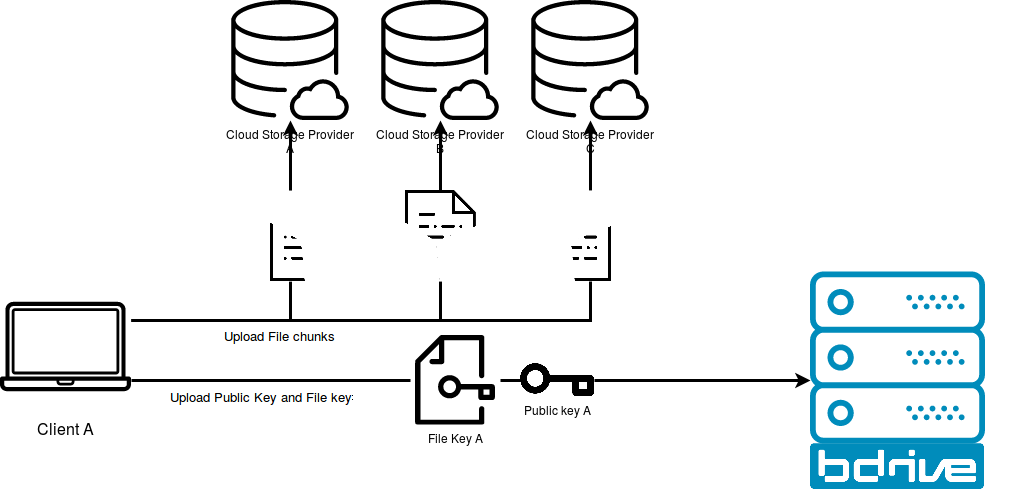
\includegraphics[width=0.8\linewidth]{img/bdrive1.png}\par 
    \caption{Client uploads an encrypted file to CSP, the file key and public key to Bdrive.}
    \label{fig:filekey}
\end{figure*}
\begin{figure*}[!ht]
\centering
    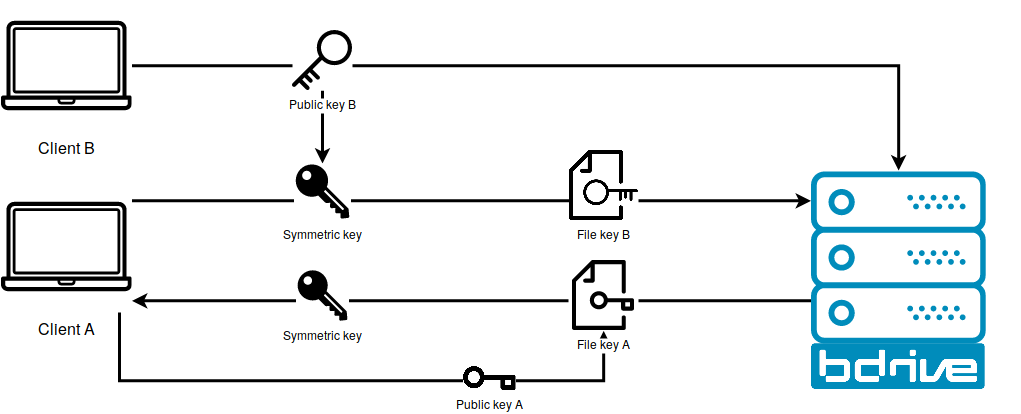
\includegraphics[width=0.8\linewidth]{img/bdrive2.png}\par
    \caption{Client A grants Client B access to the uploaded file by re-keying the file key}
    \label{fig:rekey}
\end{figure*}

%----------------------------------------------------------------------------------------

\end{document}
